%*****************************************************************************************
%*********************************** Sixth Chapter **************************************
%*****************************************************************************************

\chapter{Perovskite-coated metal islands}

\graphicspath{{Chapter6/Figures/}}

The interactions between localised surface plasmons (LSPs) and the materials in their vicinity can be utilised for a host of applications. For example, sensitivity of the resonance frequency to the local dielectric function can be exploited in sensing devices \cite{Jensen2000, Xu2004, Malinsky2001, Royer1987}, while the large field enhancements caused by electron oscillations can be used to increase Raman signals \cite{Cade2009, Olson2001, Talley2005} or emission rates \cite{Toftegaard2011, Cho2010, Reboud2013, Blanco2004}. LSP resonances of noble metal nanoparticles can be tuned across the visible spectrum via their geometries, so the fabrication of metal island nanostructures are often adjusted to suit the application.

In this Chapter the creation of Au/Ag nano-islands overcoated with a perovskite layer is described. Such systems are then used to understand light-matter coupling between excitons and LSPs, with a view to creating new quasiparticles via strong coupling.

\section{Metal island films}
Thin film morphology depends on interactions between the film and substrate atoms (i.\,e.\,the diffusion of metal atoms on substrate surface), as well as external conditions such as deposition rate, substrate temperature and subsequent annealing steps \cite{Kaiser2002}. Deposition via evaporation is a heterogeneous nucleation process, and requires high vapour pressure. Various growth modes are possible, but for noble metal films deposited on silica the metal-metal interactions are stronger than metal-substrate interactions, therefore islands are formed on the substrate \cite{Kaiser2002}. With increased deposition time islands can coalesce, either preserving the existing grain boundaries or forming a continuous structure \cite{Sennett1950,Gupta2002}.

Such metal island films (MIFs) are essentially nanoparticle arrays: if the islands are well separated (separation $l \gtrsim\,	$island diameter $d$) then there is no optical coupling between the particle resonances and we expect to see a single LSP resonance in optical spectra. The resonance wavelength of these arrays depend on the island geometry, and can be controlled by the thickness of the deposited film \cite{Walter2006, Sennett1950, Gupta2002, Gadenne2002, Lee1992}. As with nanoparticles we can model islands as dipoles embedded in a medium with dielectric function $\epsilon_d$ to predict the resonance wavelength, with care taken to include the effects of the substrate \cite{Yamaguchi1960, Yamaguchi1972, Yamaguchi1973, Doremus1966}.

\subsection{Experimental methods}
Silica substrates are prepared using the sonication steps described in Sec.\,\ref{sec:glass}. Metal deposition is performed using an Edwards resistance evaporator, under pressure $\sim4\times10^{-6}$\,mbar with deposition rate $\sim0.5$\,\AA/s. The substrates are not heated, and the deposited film thickness $t$ is determined by a 6\,MHz quartz crystal microbalance. To avoid oxidation, Ag samples are placed in a nitrogen purge dessication cabinet within 15\,minutes of fabrication, and only removed for further processing/characterisation. Annealed Au and Ag MIFs are made by heating the samples at $200^{\circ}$C for 24\,hours in vacuum. In order to create the CHPI overcoating, a CHPI/THF solution is spin coated onto the nanostructured films under a dehydrated atmosphere (layer thickness $\sim100$\,nm). The samples are then characterised using AFM, SEM and white light microscopy. During optical measurements 400 unpolarised reflection ($R$) and transmission ($T$) spectra are taken over a 0.5$\times$0.5mm$^{2}$ area and averaged to produce the data shown. Due to sample uniformity, this data is representative of the entire sample, and the absorption $A = 1 - R - T$ as scattering from these samples is less than 1\%.

\begin{figure}[h!] 
\centering    
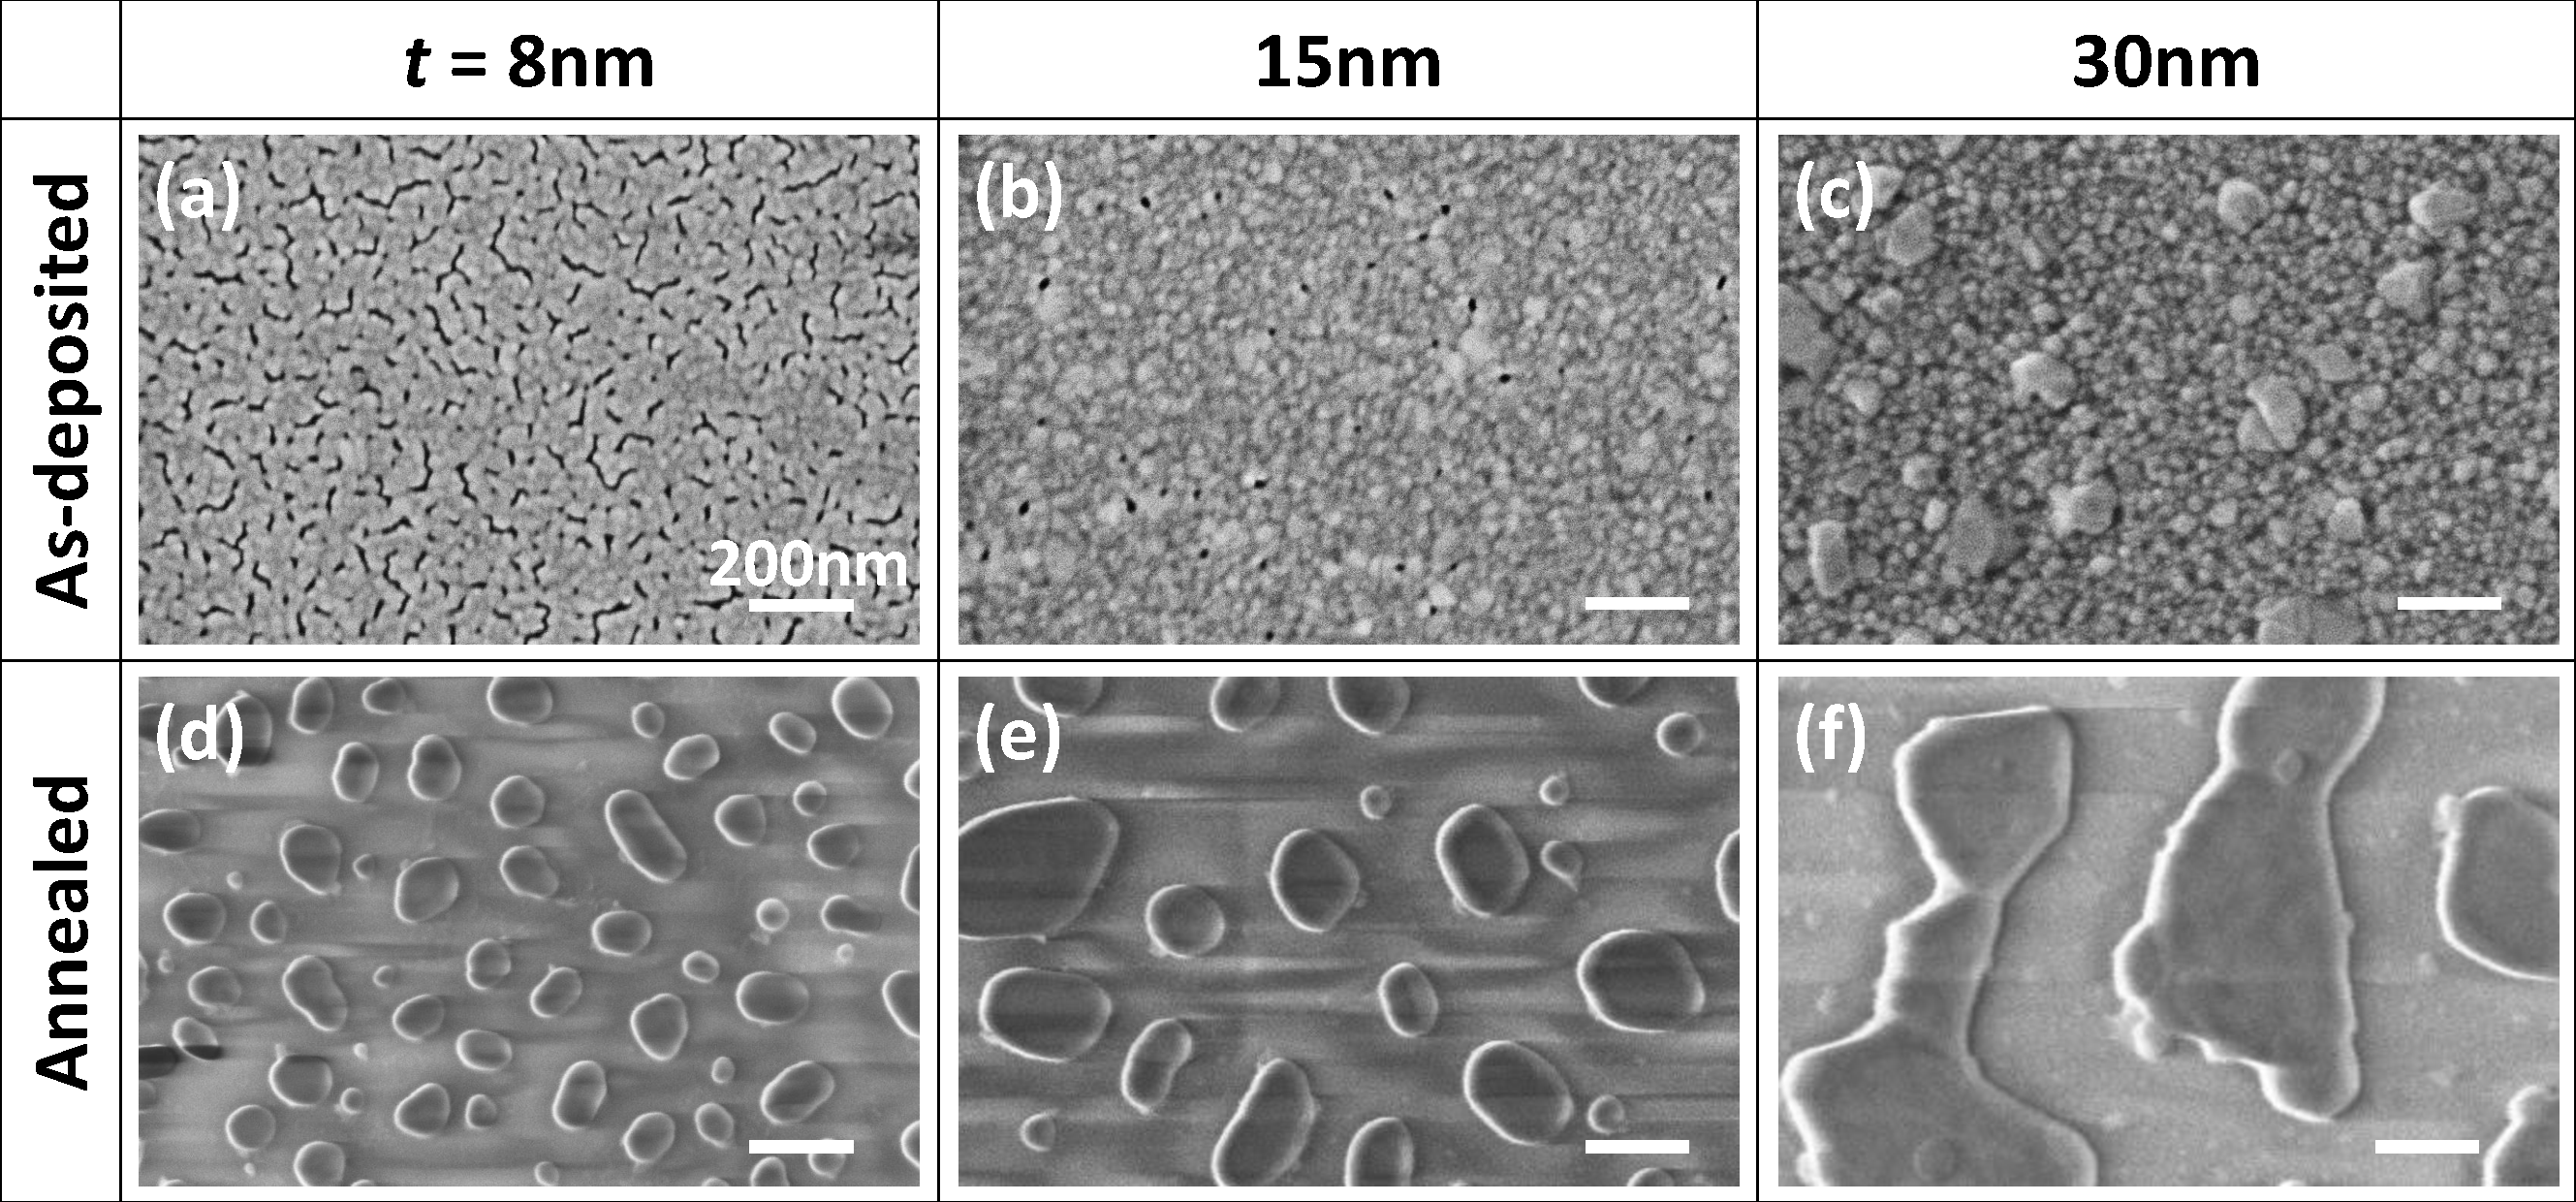
\includegraphics[width=\textwidth]{Fig1}
\caption{SEM images of (a-c) as-deposited and (d-f) annealed Au metal island films. The initial deposited film thickness $t$ is labelled.}
\label{6Fig1}
\end{figure}
\subsection{Au metal island films}

SEM images of evaporated Au films on silica show the formation of a rough but continuous film for $t=30$\,nm [Fig.\,\ref{6Fig1}(c)]. As $t$ decreases dewetting is observed as a result of weak Au-substrate interactions [Figs.\,\ref{6Fig1}(a,b)]. During annealing, Au atoms diffuse and form distinct islands [Figs.\,\ref{6Fig1}(d-f)]. With decreasing $t$ the islands become more closely spaced and ellipsoidal, smaller in both lateral size $d$ and height $h$ [Fig.\,\ref{6Fig2}]. For $t=8$\,nm we observe islands with $d \sim 50-100$\,nm, $h\sim70$\,nm, and separation $l \sim 100-200$\,nm. The decrease in island size is seen optically in 100$\times$ magnification DF reflection images, where scattering from the islands due to LSP resonances is broadband for $t=30$\,nm, but becomes progressively redder as the film thickness and island size decrease [Fig.\,\ref{6Fig2}]. 
\begin{figure}[h!] 
\centering    
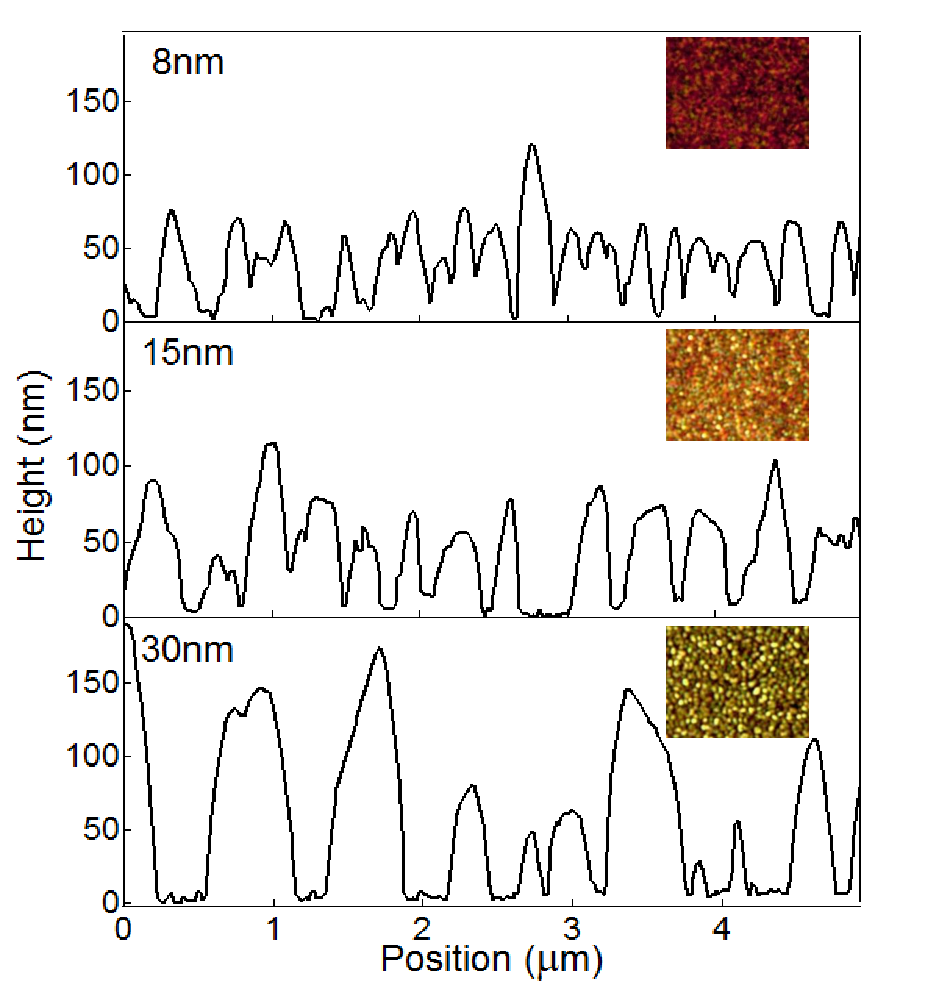
\includegraphics[width=0.85\textwidth]{Fig2}
\caption{AFM profiles of annealed Au metal island films. The deposited film thickness $t$ is labelled. Insets show 100$\times$ magnification DF images of the samples.}
\label{6Fig2}
\end{figure}

Fig.\,\ref{6Fig3} shows the absorption spectra for $t=8$\,nm as-deposited and annealed Au MIFs. We observe a resonance $\lambda_{dep} = 570$\,nm in the absorption of the as-deposited film, however this is due to grains in the film and therefore has a large linewidth $\Gamma_{dep} = 245$\,nm. In the annealed film we observe a resonance $\lambda_{anneal} = 550$\,nm with linewidth $\Gamma_{anneal} = 50$\,nm due to island LSPs.

\begin{figure}[h!] 
\centering    
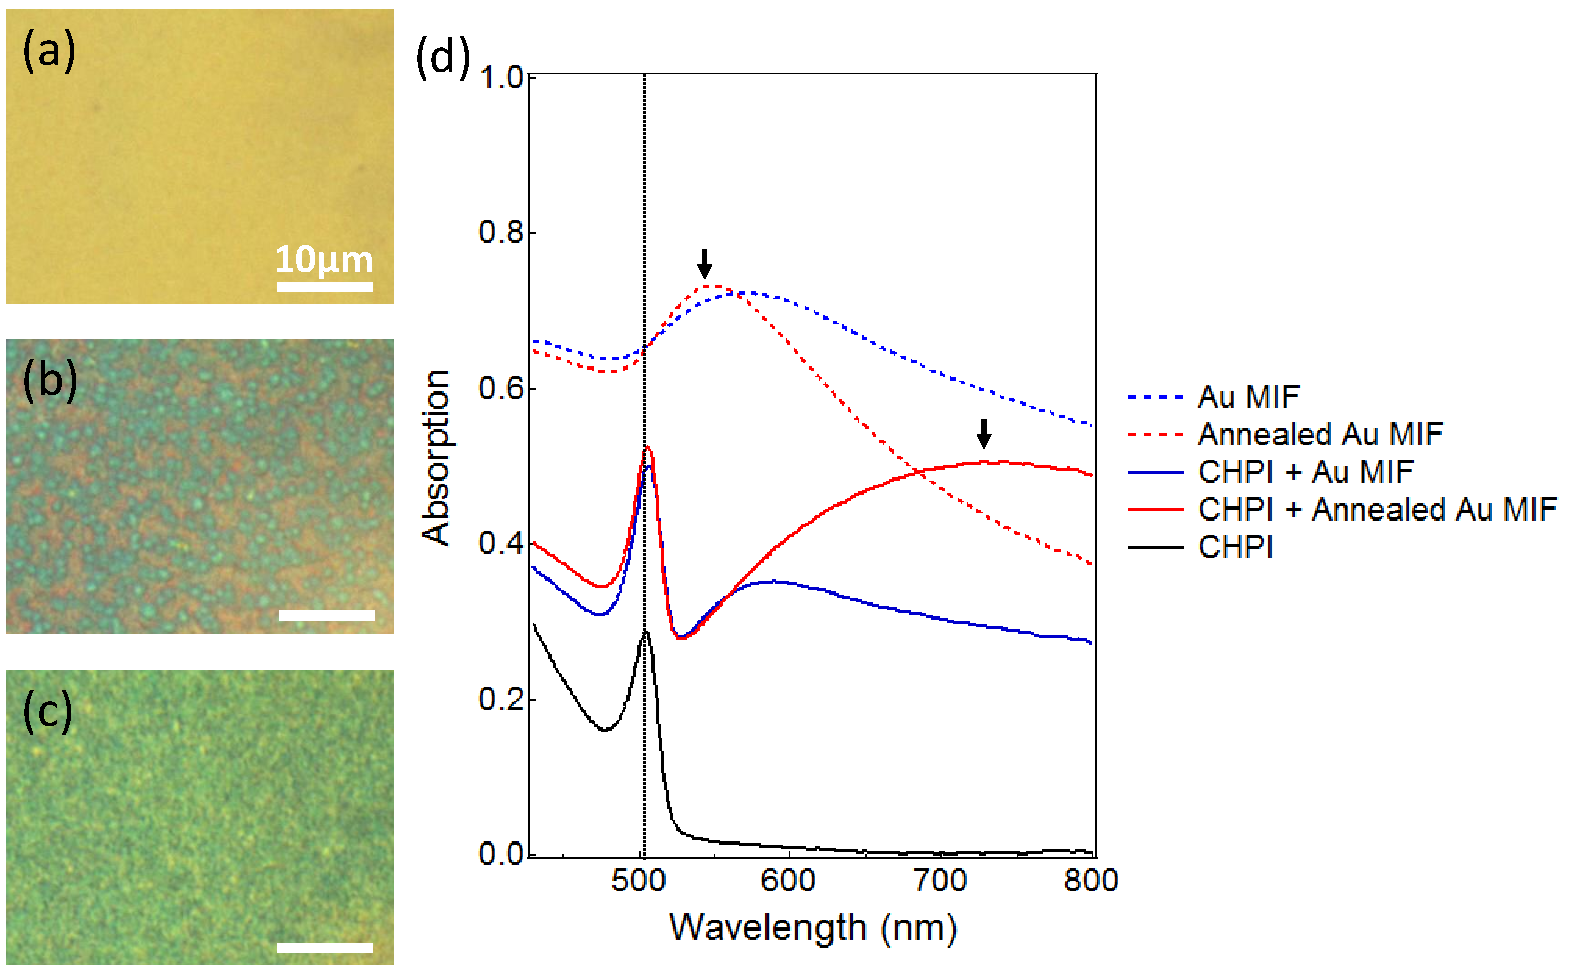
\includegraphics[width=\textwidth]{Fig3}
\caption{BF images at 100$\times$ magnification for CHPI films on (a) silica, (b) $t=8$\,nm as-deposited and (c) $t=8$\,nm annealed Au metal island films. (d) Average absorption spectra for 400 pixels over $0.5\times0.5$\,mm$^2$. The exciton wavelength is marked by the dashed line, and LSP resonances by arrows. The (annealed) Au MIF spectra are offset for clarity.}
\label{6Fig3}
\end{figure}
\subsection{CHPI-coated Au metal island films}

BF reflection images at 100$\times$ magnification show the formation of CHPI on silica [Fig.\,\ref{6Fig3}(a)] and $t=8$\,nm as-deposited and annealed Au MIFs [green areas in Figs.\,\ref{6Fig3}(b,c)]. The exciton resonance $\lambda_{ex} = 505$\,nm is observed for all three films, confirming formation of the MQW structure despite some roughness and dewetting on Au substrates. We observe a redshift in the LSP resonance as a result of the CHPI coating ($\lambda_{anneal} = 550$\,nm $\rightarrow 735$\,nm), with a considerable increase in the linewidth due to the non-uniform CHPI coverage ($\Gamma_{anneal} = 50$\,nm $\rightarrow 200$\,nm). However the excitons in CHPI are completely unaffected by the presence Au islands as the two oscillations are far off-resonance, so the exciton peak remains at the same wavelength and linewidth. The overall magnitude of the absorption across the entire visible range has increased as a result of absorption by the metal film.
%CHPI+annealed Au LSP linewidth ~500nm+?

\begin{figure}[h!] 
\centering    
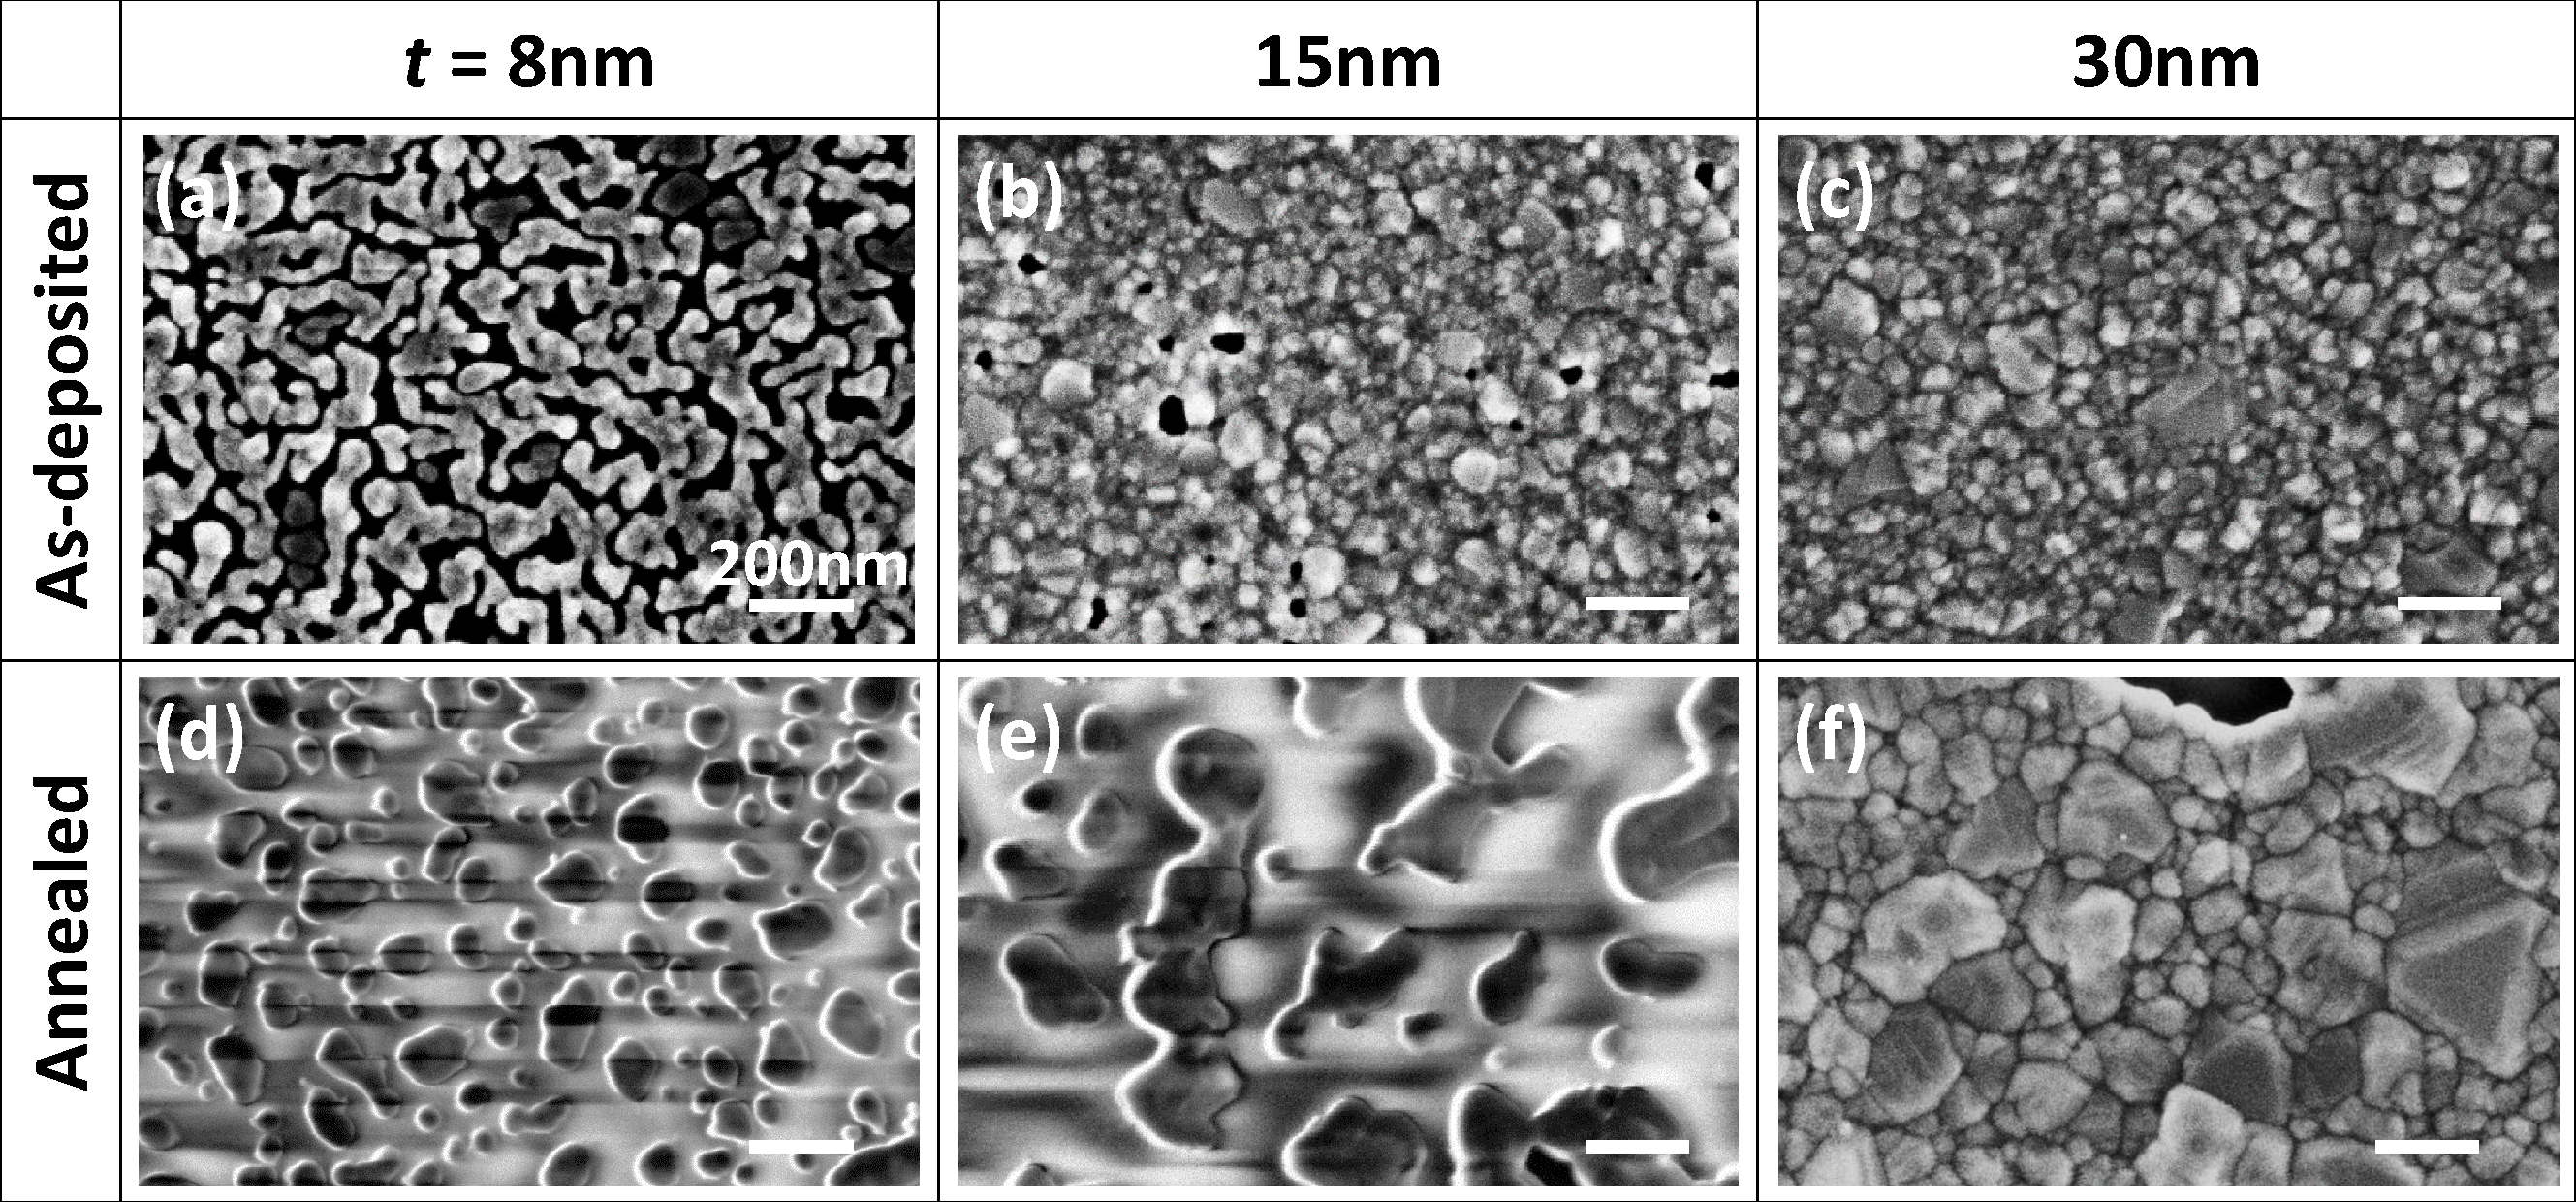
\includegraphics[width=\textwidth]{Fig4}
\caption{SEM images of (a-c) as-deposited and (d-f) annealed Ag metal island films. The initial deposited film thickness $t$ is labelled. Dark areas/streaks in (a, d, e) are due to charging of the sample.}
\label{6Fig4}
\end{figure}
\subsection{Ag metal island films}

The morphology of evaporated Ag films on silica are similar to Au: rough films lead to dewetting with decreasing $t$, as well as formation of MIFs when the as-deposited films are annealed [Fig.\,\ref{6Fig4}]. However the Ag-substrate interactions are stronger as annealing does not cause island separation for $t=30$\,nm films, only an increase in grain size. Annealed $t=8$\,nm Ag MIFs consist of ellipsoidal islands with $d \sim40-100$\,nm, $h\sim80$\,nm, and $l\sim50-150$\,nm [Fig.\,\ref{6Fig5}]. DF images at $100\times$ magnification also show a change from broadband white scattering to green as $t$ decreases [Fig.\,\ref{6Fig5}]. 

\begin{figure}[h!] 
\centering    
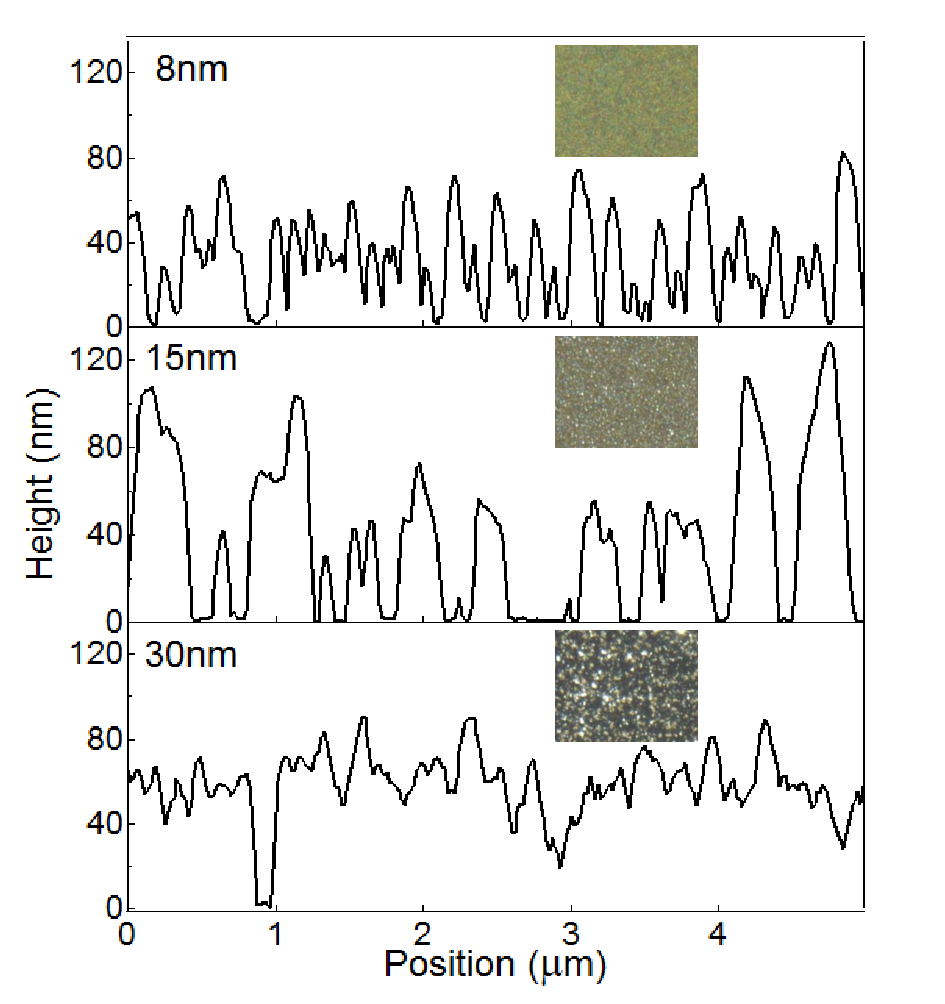
\includegraphics[width=0.85\textwidth]{Fig5}
\caption{AFM profiles of annealed Ag metal island films. The deposited film thickness $t$ is labelled. Insets show 100$\times$ magnification DF images of the samples.}
\label{6Fig5}
\end{figure}

As seen in the SEM images, as-deposited Ag films are essentially continuous with some dewetting if $t>8$\,nm. Thus absorption spectra are similar to that of bulk Ag films, with an increase in absorption up to the band gap $\sim300$\,nm [Fig\,\ref{6Fig6}(a)]. However resonances can be observed for lower $t$, particularly $t=2$\,nm ($\lambda_{dep} = 560$\,nm, $\Gamma_{dep} = 175$\,nm), indicating formation of islands even without annealing [see also Sec.\,\ref{sec:AgonCHPI}]. 

After annealing, LSP resonances of Ag islands dominate the absorption spectra [Fig.\,\ref{6Fig6}(b)]. Although the positions of the absorption peaks do not change significantly with $t$, there is a clear decrease in the linewidth of the $t=2$\,nm film compared to the others [Fig.\,\ref{6Fig6}(c)]. The relative stability of the LSP wavelength suggests the average island size does not change with $t$. However we may have a larger range of island shape/size for thicker films, leading to a superposition of many resonance wavelengths and higher order LSP modes, and an apparent increase in the LSP linewidth.
\begin{figure}[h!] 
\centering    
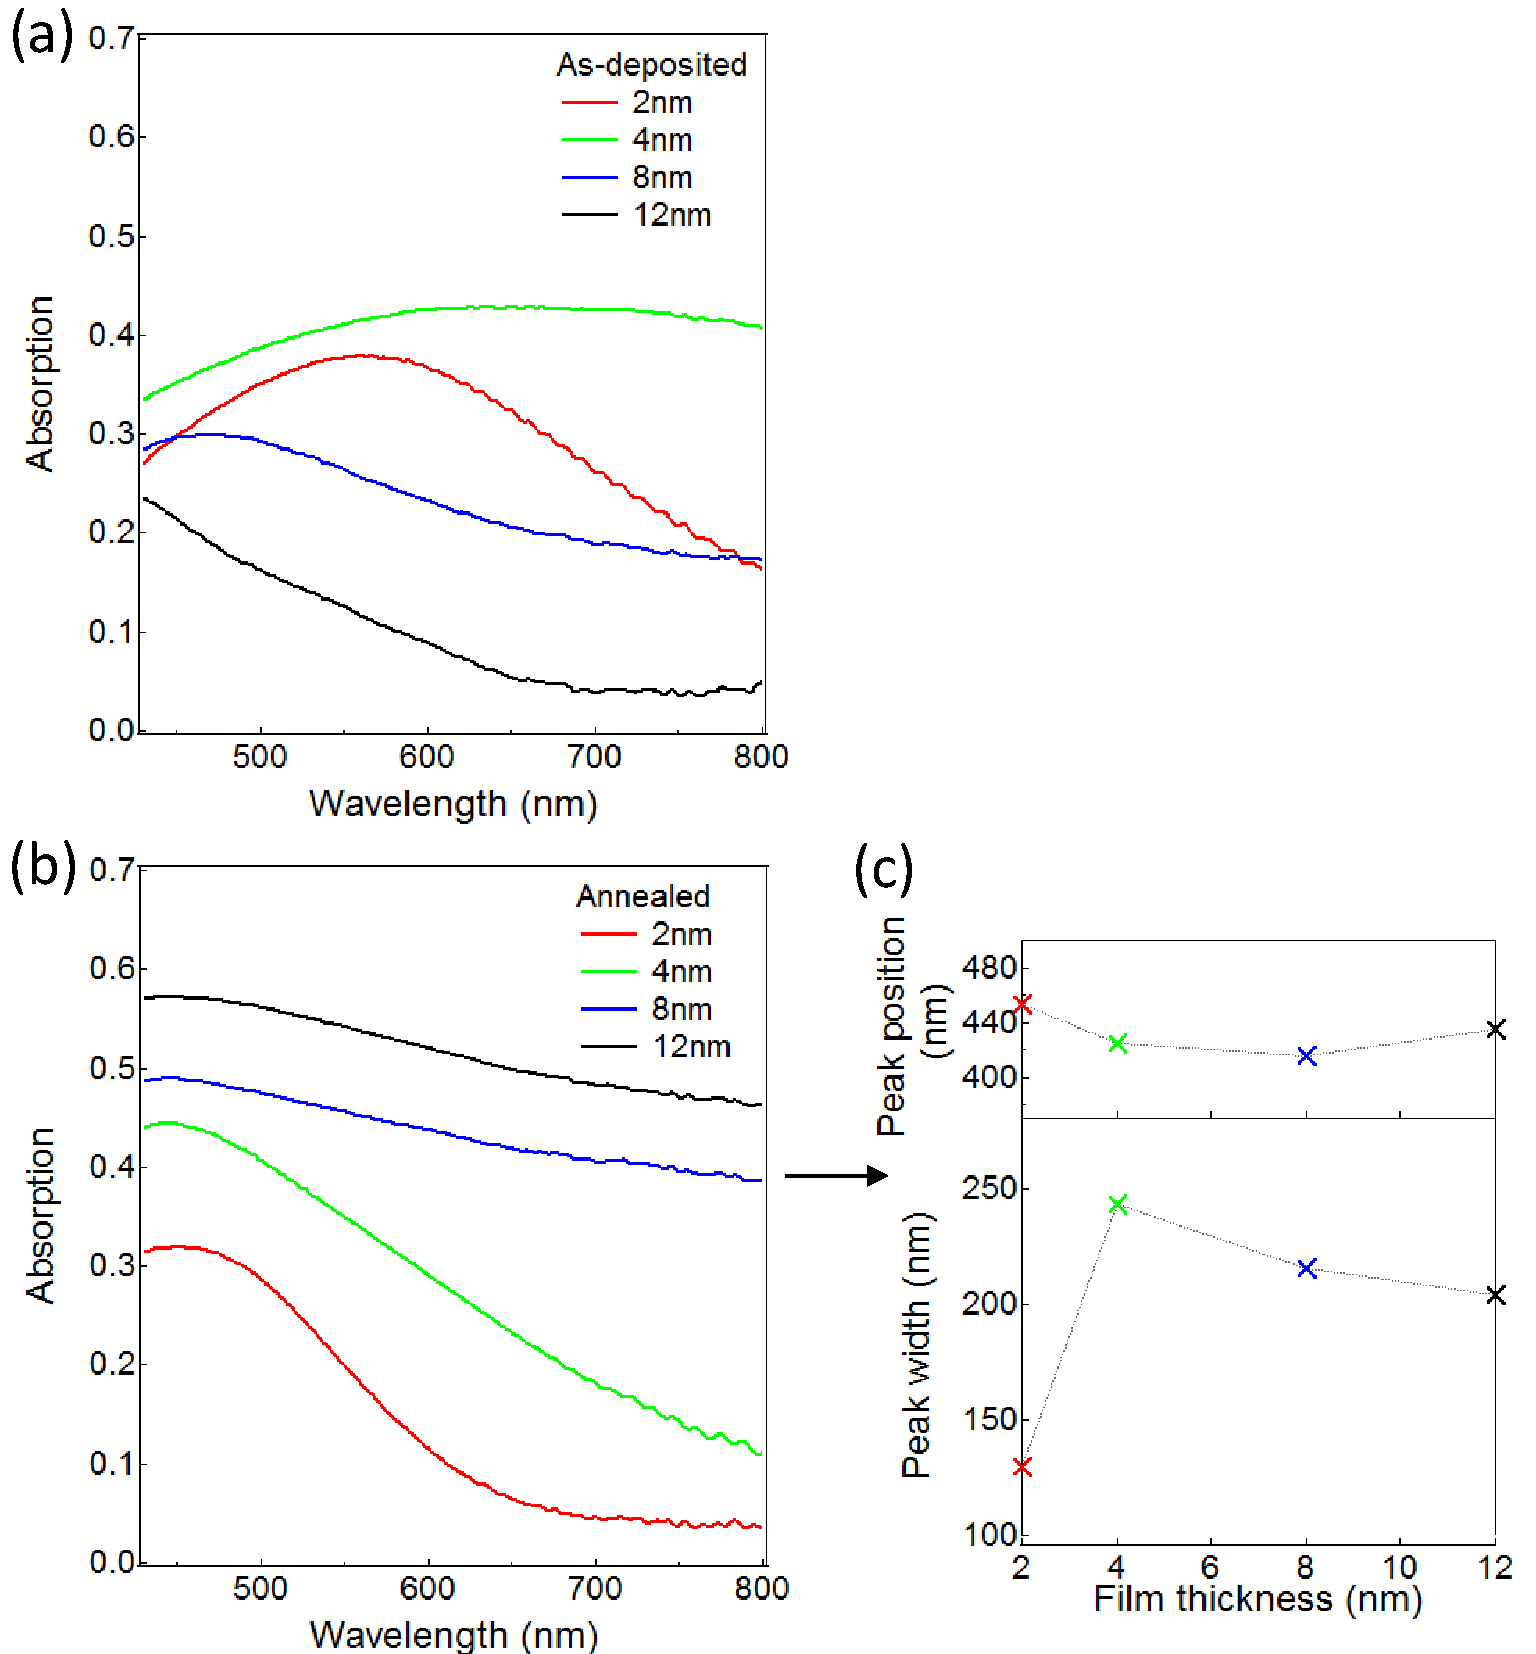
\includegraphics[width=\textwidth]{Fig6}
\caption{Average absorption spectra for 400 pixels over $0.5\times0.5$mm$^2$ for (a) as-deposited and (b) annealed Ag metal island films with the thickness $t$. (c) Absorption peak position and linewidth for the spectra in (b).}
\label{6Fig6}
\end{figure}

\subsection{CHPI-coated Ag metal island films}
\label{sec:CHPI_AgMIF}
\begin{figure}[h!] 
\centering    
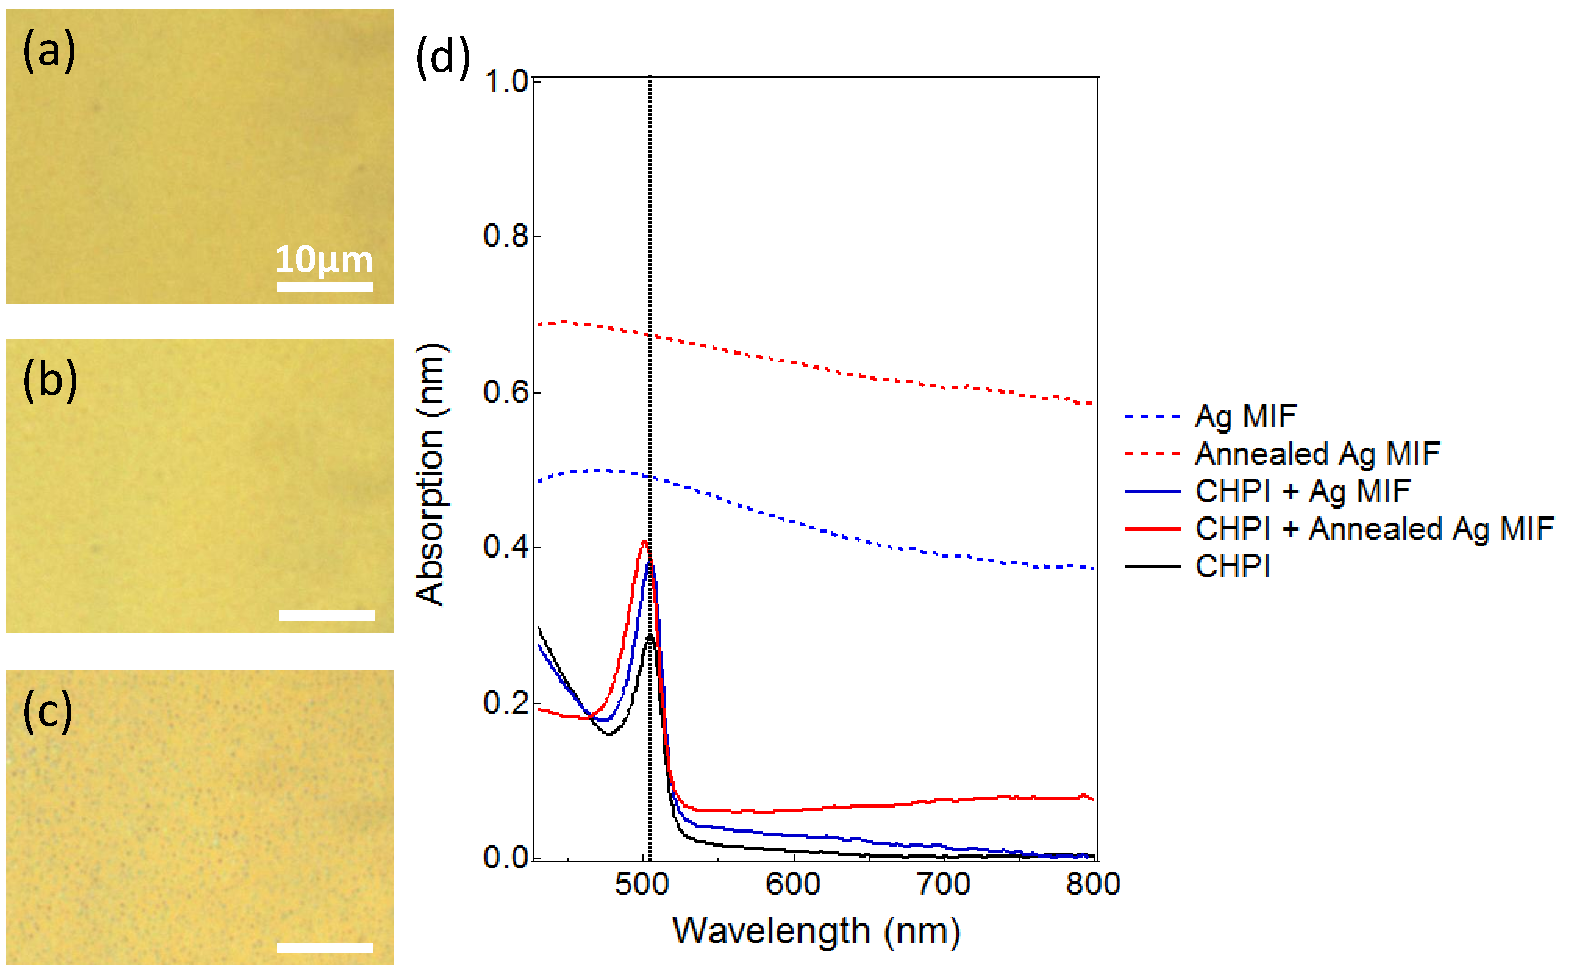
\includegraphics[width=\textwidth]{Fig7}
\caption{BF images at 100$\times$ magnification for CHPI films on (a) silica, (b) $t=8$\,nm as-deposited and (c) $t=8$\,nm annealed Ag metal island films. (d) Average absorption spectra for 400 pixels over $0.5\times0.5$mm$^2$. The exciton wavelength of the CHPI film on silica is marked by the dashed line. The (annealed) Ag MIF spectra are offset for clarity.}
\label{6Fig7}
\end{figure}
%WN
Due to similarities in the LSP resonances, CHPI-coated Ag films behaved in the same manner for $t\leq8$\,nm, and here we use $t=8$\,nm as an example. %end
BF images at 100$\times$ magnification show very little difference between CHPI films on silica, as-deposited or annealed Ag MIFs [Fig.\,\ref{6Fig7}(a-c)], although some non-uniformity is observed in the case of the annealed Ag MIF. From the optical spectra in Fig.\,\ref{6Fig7}(d), we can see that as-deposited Ag MIFs cause little change to the exciton wavelength and linewidth, although the absorption has increased by 33\%. However for annealed Ag MIF the island LSP shifts to $\sim550$\,nm due to the CHPI coating and overlaps with the exciton resonance. Thus we see weak coupling in the form of a blueshift in the exciton wavelength by 5\,nm  ($\lambda_{ex}=500$\,nm), as well as an enhancement of the exciton absorption peak by 42\%. Coupling-induced enhancement of semiconductor absorption due to LSP field enhancements is a well-known phenomenon \cite{Balci2014, Alemu2014, Zheng2011, Xu2013, Spinelli2012}, however we were unable to observe modification of the exciton wavefunction via strong coupling as the LSP is not fully resonant with the exciton.

\subsection{Ag islands on CHPI films}
\label{sec:AgonCHPI}

Instead of coating Ag MIF films with CHPI, we also fabricated samples of Ag islands deposited on a CHPI film on silica. Since the CHPI organic molecules undergo a melting transition $\sim$80$^{\circ}$C \cite{Barman2003}, we thermally evaporate only 2\,nm of Ag to prevent degradation of the CHPI film due to heat. The AFM profile of a 2\,nm as-deposited Ag MIF on silica [Fig.\,\ref{6Fig8}(b)] shows the formation of separated metal islands, with $d\sim30$\,nm and $h\sim6$\,nm, %WN
however this measured height is likely due to the AFM tip not reaching the substrate as a result of its finite radius ($\approx 100$\,nm). %end
The AFM profile of an Ag MIF on CHPI is dominated by surface roughness of the CHPI film ($\sim$5\,nm, \textit{cf} Fig.\,\ref{6Fig8}(a)), however some high frequency noise on the order of $d$ can also be seen. The lack of distinct MIF features suggests Ag islands may be partially embedded in the CHPI film. However the thermal evaporation of Ag has not significantly damaged the CHPI film as a strong exciton peak can still be seen in absorption spectra [Fig.\,\ref{6Fig8}(d)]. In the same way as Sec.\,\ref{sec:CHPI_AgMIF}, the Ag island LSPs have again weakly coupled to excitons, causing a blueshift of 4\,nm but an increase in absorption of only 9\% in this case [Fig.\,\ref{6Fig8}(d)].
\begin{figure}[h!] 
\centering    
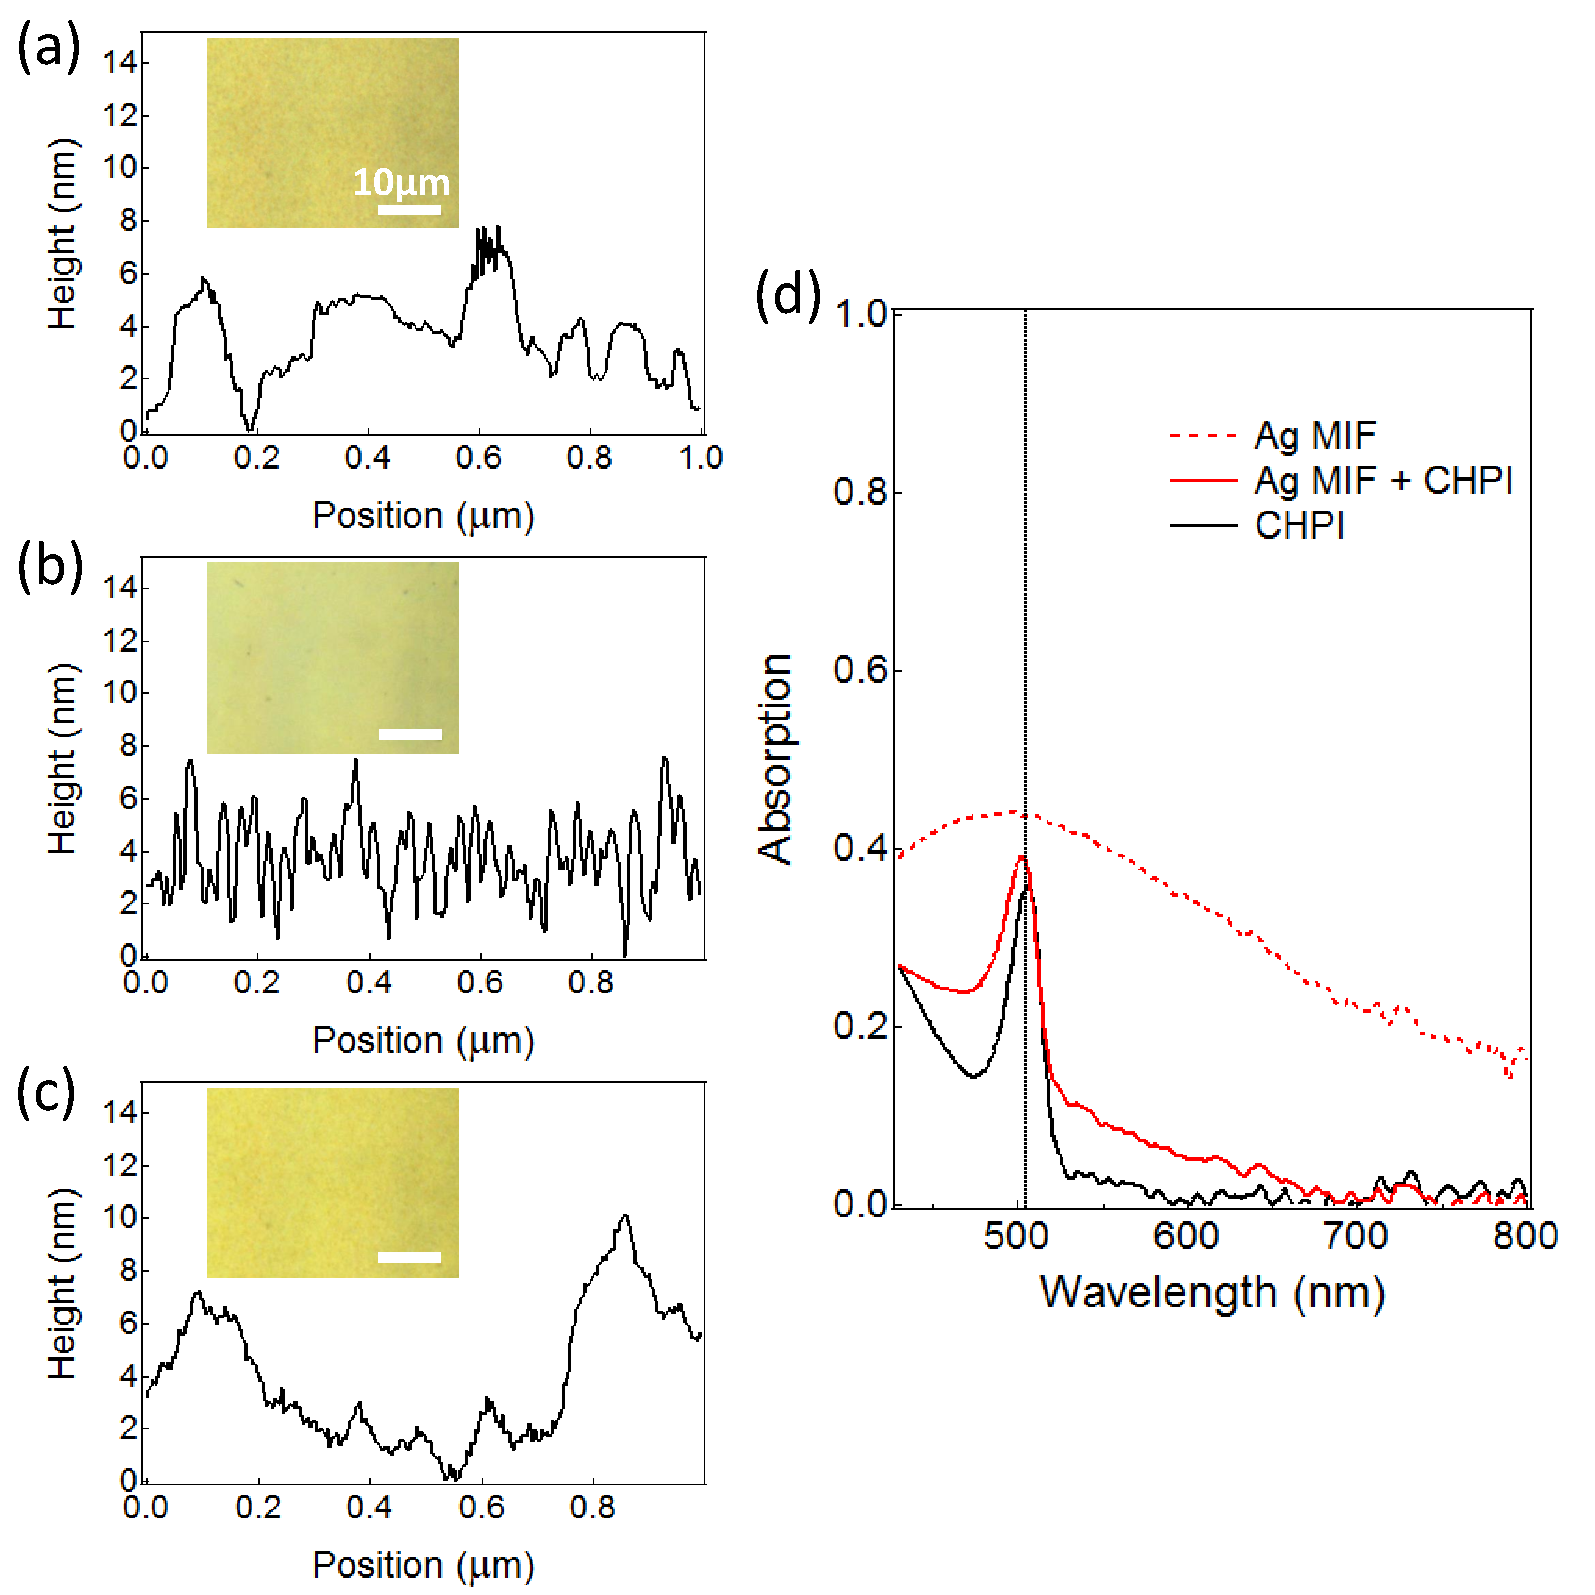
\includegraphics[width=\textwidth]{Fig8}
\caption{AFM profiles of (a) CHPI film on silica, (b) $t=2$\,nm evaporated Ag film on silica, and (c) $t=2$\,nm evaporated Ag film on CHPI. Insets show 100$\times$ magnification BF images of the samples. (d) Average absorption spectra for 400 pixels over $0.5\times0.5$mm$^2$. The exciton wavelength of the CHPI film on silica is marked by the dashed line. The Ag MIF spectrum is offset for clarity.}
\label{6Fig8}
\end{figure}

\section{Nanosphere lithography (NL)}
Nanosphere lithography involves the evaporation of metals through closely-packed 2D arrays of nano-/microparticles followed by removal of the spheres, leaving behind an array of metal islands on the substrate \cite{Haynes2001}. NL island array geometry depends on the diameter of spheres $D$. For a colloidal monolayer, the island diameter is $0.223D$, while the inter-island separation is $0.58D$ \cite{Hulteen1995}. The interstices between spheres lead to formation of triangular islands, however for small $D$ the islands can become more spherical \cite{Hulteen1999}. Array geometry can also be controlled by the metal evaporation angle \cite{Haynes2002}.

Much like MIFs, these triangular NL islands produce an LSP peak in optical spectra that depends on the size/shape of islands as well as the dielectric environment \cite{Jensen2000}, and can be modelled as an array of dipoles \cite{Malinsky2001, Jensen1999}. However nanosphere lithography provides better control of the island geometry due to the lithography mask, and should provide a sharper LSP resonance compared to MIFs.

\begin{figure}[h!] 
\centering    
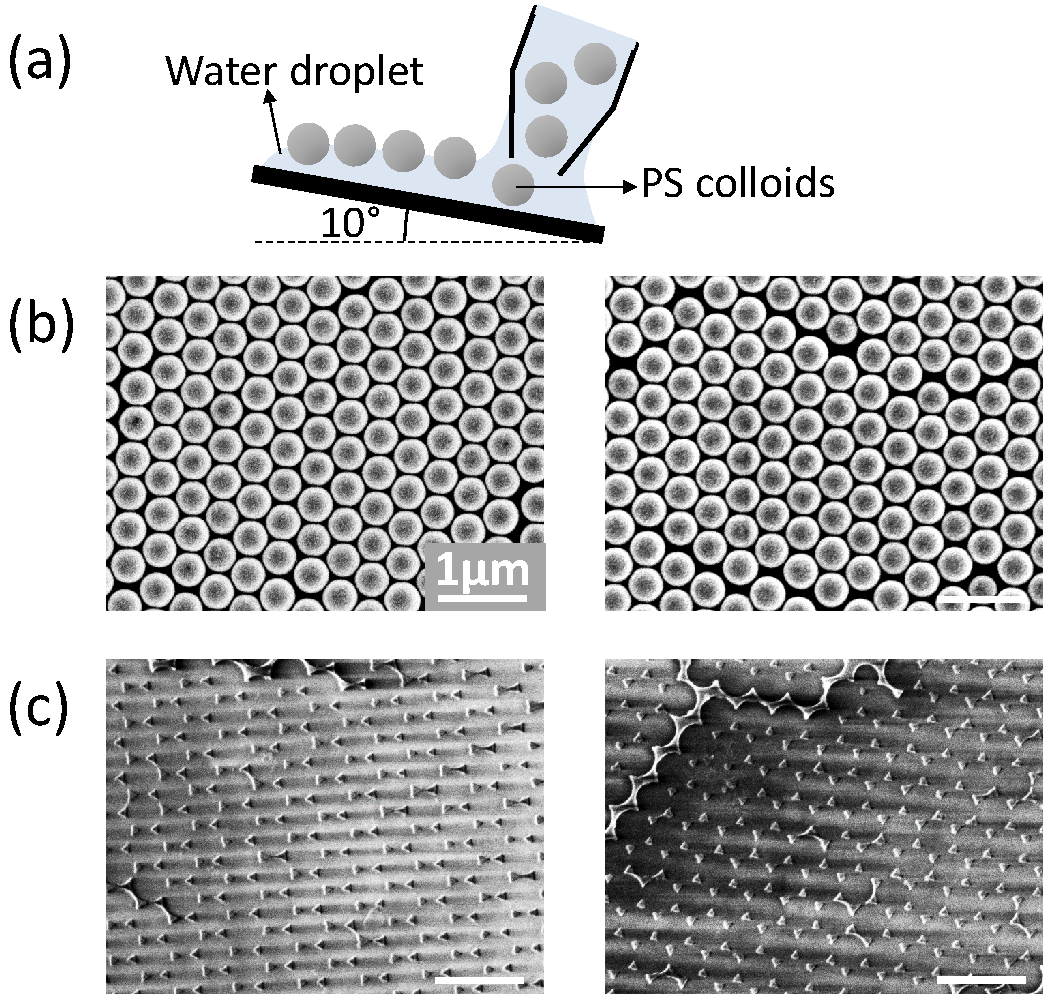
\includegraphics[width=0.8\textwidth]{Fig9}
\caption{(a) Schematic of the creation of PS colloidal monolayers on a water droplets. SEM of (b) colloidal monolayer formed after the evaporation of water, and (c) triangular islands formed after the evaporation of Au and removal of colloids.}
\label{6Fig9}
\end{figure}
\subsection{Experimental methods}
We use $D=460\pm10$\,nm polystyrene (PS) microspheres from Sigma Aldrich to create the colloidal monolayer. The 10\,vol\% microsphere solution in water is diluted in a 1:1 mix with ethanol (absolute). Silica substrates are cleaned %WN
using the sonication steps %end
described in Sec.\,\ref{sec:glass} then plasma etched for 1\,minute to create a hydrophilic surface. The substrates are placed at a $10^{\circ}$\,angle before a deionised water droplet is applied to cover the silica surface. A 2\,wt\% solution of sodium dodecylsulphate in water ($<0.5\,$\textmu l) is applied to the water surface, where the amphiphilic molecules act to reduce the surface charge on PS microspheres. A pipette is used to spread PS microspheres onto the droplet surface [Fig.\,\ref{6Fig9}(a)], and the water is allowed to evaporate under standard conditions. 50\,nm of Au is then deposited on the samples using an electron-beam evaporator system under pressure $\sim5\times10^{-6}$\,Torr at a rate of 1\AA/s. The PS microspheres are dissolved by placing the sample in a solution of dichloromethane for 30\,minutes, then sonicating the solution for 5\,minutes. Finally, a CHPI/THF solution is spin coated onto the island samples under a dehydrated atmosphere. Optical characterisation is performed by taking 400 scans over a $50\times50\,$\textmu m$^{2}$ region, then averaged to produce the spectra shown. 

\subsection{Au NL islands}
Closely-packed 2D arrays of PS microspheres are formed using this technique [Fig.\,\ref{6Fig9}(b)], and the ordering is best at contact lines of the solution. After the removal of PS, triangular islands are left behind on the silica substrate [Fig.\,\ref{6Fig9}(c)] with $d\sim90$\,nm. We can see from Fig.\,\ref{6Fig9}(c) that even in the best areas we do not find uniformly well-separated triangular islands. Due to small variations in the microsphere packing bow-tie shaped islands can form, and lines of Au are found at domain boundaries. However in the absorption spectra of such island samples [Fig.\,\ref{6Fig10}] we do observe an LSP resonance at 590\,nm with a linewidth of 80\,nm, comparable to MIF spectra.

\subsection{CHPI-coated Au NL islands}
Similar to CHPI-coated Au MIFs, strong exciton peaks in the absorption spectra of CHPI-coated Au NL islands indicate formation of the MQW structure. The exciton wavelength is unaffected by the Au ($\lambda_{ex} = 505$\,nm). As before, the LSP resonance redshifts due to the CHPI coating, and the linewidth broadens to $\sim$150\,nm. We observe a systematic increase of the LSP redshift as a result of increasing spin speed, and attribute this to more complete CHPI encapsulation of the Au islands as a result of larger forces at high spin speeds.
\begin{figure}[h!] 
\centering    
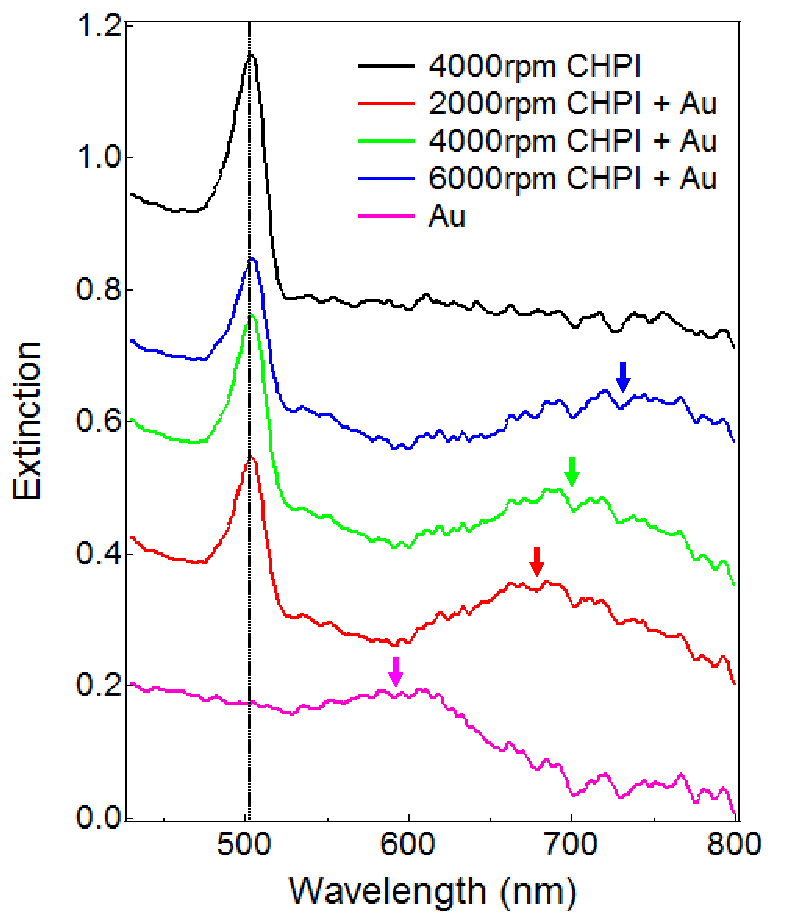
\includegraphics[width=0.7\textwidth]{Fig10}
\caption{Average absorption spectra for 400 pixels over $50\times50\,$\textmu m$^2$ of CHPI-coated Au nanosphere lithography islands. Arrows indicate the positions of LSP resonances, and the dashed line indicates the exciton wavelength. The spectra are offset for clarity.}
\label{6Fig10}
\end{figure}

\section{Conclusions}
Evaporation of noble metals can be %WN
used %end
to create ellipsoidal nanoparticles on a silica substrate. These metal island films behave like a nanoparticle array, and show distinct LSP resonances that can be tuned via deposition parameters. In the case of perovskite-coated Au islands the LSPs are far off-resonance with excitons, and the dielectric coating causes a redshift of the LSP peak with no effect on excitons. In the case of perovskite-coated Ag islands, LSPs weakly couple to excitons and cause a blueshift in the exciton resonance of 5\,nm, as well as an increase in exciton absorption by $\sim40$\% due to the electric field enhancement. Such enhancement has been investigated and is of particular interest for the design of solar cells \cite{Alemu2014, Zheng2011, Xu2013, Spinelli2012}.

The linewidth of the LSP resonance may be a barrier to strong coupling between plasmons and excitons in perovskite-coated nanostructures. The large variation in shape and size of metal particles in MIFs is an issue, however from our experiments the more controllable island geometries created using nanosphere lithography do not show a marked improvement in LSP linewidth. Chemically created metallic NPs, which are often pre-screened for size, may provide an avenue for future exploration, however a method of controllably assembling a dense array of well-separated NPs from solution will need to be investigated.